\chapter{Introduction}


These exercises in the Web Ontology Language (OWL) take participants through OWL from its basics to some rather advanced features of the OWL~DL profile of OWL. The exercises use family history as a topic and much of the tutorial is based on the `Manchester Family History Advanced OWL Tutorial' found at \url{http://owl.cs.manchester.ac.uk/publications/talks-and-tutorials/fhkbtutorial/}. Here, instead of an `advanced tutorial', the exercises go from the start to quite a lot of what anyone using OWL to model needs to know about the language and the use of an automated reasoner; the exercises do not really explore much in the way of modelling issues.	 

These exercises don't give any instruction in \protege; for that use the Pizza tutorial at \url{http://owl.cs.manchester.ac.uk/tutorials/protegeowltutorial/}. These exercises don't give any explanation behind the phenomena revealed during the exercises; these are explained by the human beings delivering the exercises. More explanation can be found in the Pizza tutorial and the written, original, long version of the Family History OWL tutorial is in Blackboard.

In these exercises we take an ``objects (individuals) first'' approach. Most tutorials concentrate on classes then individuals (if at all). By doing it this way our aim is to emphasise  that OWL is all about modelling individuals--even if most axioms are restrictions upon classes that say `each and every individual in this class holds at least one of these properties to an individual of the filler class'. Similarly, object properties are relationships between two individuals, we just usually model at the class level and these sort of distinctions can sometimes get lost. So, these exercises start with asserting lots of properties between named individuals and only later do we start talking about classes of these individuals. It may be, and probably will be, that most modelling is with classes and properties, but this way really emphasises what the language is actually doing.

Subsequent material in the course unit will focus largely on classes and modelling with classes. 

Once you have completed these exercises in the lab, you are recommended to work your way through the Protege Pizza tutorial and the Family History OWL Tutorial. These will help you gain experience of the mechanics of using \protege and provide a further introduction to \owlii. 

\begin{itemize}
\item \url{http://owl.cs.manchester.ac.uk/tutorials/protg-owl-tutorial/}
\item \url{http://owl.cs.manchester.ac.uk/publications/talks-and-tutorials/fhkbtutorial/} contains the ontologies, and the long version of the tutorial explanation is in Blackboard. 
\end{itemize}

\section{Learning outcomes}

By the end of a successful completion of these exercises you should be able to:

\begin{enumerate}
\item Understand the core aspects of \owlii syntax and semantics;
\item Use \protege to build an ontology, and use an automated reasoner to draw inferences from the axioms in your ontology;
\item Use classes and individuals;
\item Use \owlii's property hierarchy;
\item Use \owlii's property characteristics;
\item Know more than you need to about the famly history of \rds;
\item Know some of the limitations of \owlii.
\end{enumerate}
\noindent These learning outcomes are very generic; each exercise encapsulates a significant learning outcome. For example, Exercise~\ref{ex:date} has a learning outcome of: knowing how to use data properties; knowing about and using the \con{DifferentIndividuals} axiom; a reinforcement of the use of the functional property characteristic; and an introduction to qualified cardinality restrictions.

\section{Assumptions}


We make some simplifying assumptions in this tutorial:
\begin{itemize}
\item We assume people doing the exercises know nothing about OWL.
\item We assume that there are human beings present that are knowledgeable about OWL to conduct participants through the exercises and give explanations. You may need to ask these human beings (or consult some other sources) to understand some of the terms used in this tutorial (e.g., ``inverse'' or ``transitive''). 
\item We take a conventional western  view of family history. This appears to have most effects on naming of sibling and cousin relationships.
\item We take a straight-forward view on the sex of people; this is explored further in Chapter~\ref{ex:sex};
%\item A 'conventional' view of marriage is taken; this is explored further in Chapter~\ref{chap:marriage}.
\item We make no special treatment of time or dates; we are only interested in years and we do not do anything fancy; this is explored more in Chapter~\ref{ex:date}.
\end{itemize}
At the end of the tutorial, you should be able to produce a property hierarchy and a TBox or class hierarchy; all supported by use of \protege, the automated reasoner, and a lot of \owlii's features.

% At the end of the tutorial, you should be able to produce a property hierarchy and a TBox or class hierarchy  such as shown in Figure~\ref{fig:class_and_prop_hierachy}; all supported by use of the automated reasoner and a lot of \owlii's features.

% \begin{figure}
% \begin{center}
% 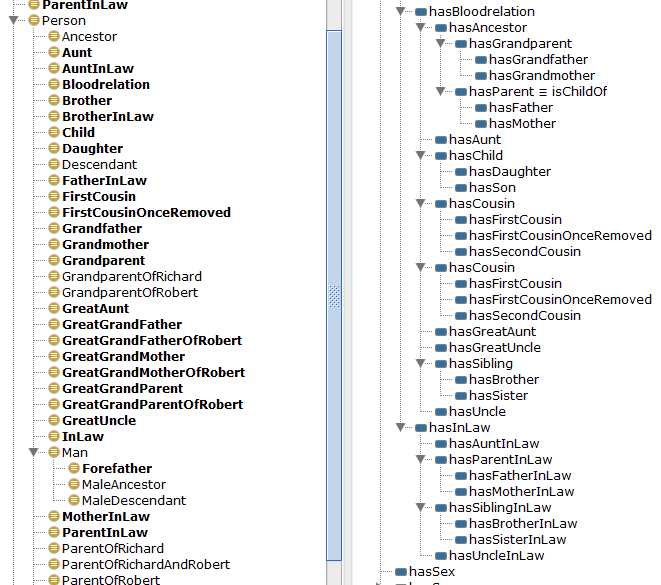
\includegraphics[width=\largefigwidth]{figures/class_prop_hierachy_final}\caption{A part of the class and property hierarchy of the final \fhkb.}\label{fig:class_and_prop_hierachy}
% \end{center}
% \end{figure}


\section{How to use these exercises}

Start at exercise one and work through to the last exercise. Don't just read the exercises and think you know what will happen; actually do it and you'll learn more. 